%!TeX root=../Dissertation.tex
%!TeX bibfile=./analysis.bib
%!TeX bibfile=./synthesis.bib

\chapter{Review of Virtualisation}
\label{chap:virtualisationReview}

\section{Terminology \& Definitions}


\subsection{Virtualisation}
Virtualisation as a term originated in the 1960s when IBM workers began work on a project that would allow an IBM model-40 computer to segregate off its memory and allow up to 15 users to use the computer independently at once \citep{Lindquist1966}. Each user would see their own abstract Operating System, separate from the others. Whilst virtualisation has continued in its development from this point onwards, the core functionality and architecture behind Hardware Virtualisation, remain much the same.

Each of these individual logical (as opposed to physical) devices is called a `virtual machine'.

\subsection{Hardware Virtualisation}
\label{subsec:HardwareVirtualisation}
There are a number of different types of virtualisation. This can open the scope for what can and can not be considered virtualisation, so we must be firm on our definition here. For the purpose of this report the term `virtualisation' will refer specifically to `hardware based virtualisation', whereby a `virtual machine' is an operating system running on top of another operating system, with the virtualisation tasks being controlled by a `hypervisor' (This is explained in more detail in the next subsection: \ref{subsec:hypervisor}).

This is an important definition to clarify, as sometimes containerisation (Chapter \ref{chap:containerisationReview}) can be viewed as a type of virtualisation (due to the similarities of what they provide). For the purposes of this report, the two definitions must be distinguished as separate things, much like in the report ``Autonomic Orchestration of Containers: Problem Definition and Research Challenges'' \citep{casalicchio2016}, where a clear and defined difference between Hardware Virtualisation and Containerisation is made. In the following sections we shall provide more in-depth description of what a virtualisation is, and what containerisation is, so as to reduce any possible confusion.

\subsection{Host Machine}
Though this applies to containerisation also, it is important to define the host-machine here. The host-machine is the bare-metal physical machine that runs instances (whether that be virtual machines or containers). The host-machine Operating System (OS) is the OS that is installed at the lowest level on the hardware.

\subsection{Hypervisor}
\label{subsec:hypervisor}
Hardware Virtualisation relies on an underlying software that runs on the host-machine's Operating System in order to manage each instance/OS. This software can have a number of different names depending on the origin of the work, and the context. In early work on virtualisation, this software was often referred to simply as a ``control program'' \citep{creasy1981}, but for the purposes of this research, this software will be referred to as a `Hypervisor'. This term is often preferred in practical settings, such as in VMware's online Glossary \citep{vmwareHypervisor}, or in Red Hat's ``What is a hypervisor'' \citep{redhat2021}, and has become the de-facto term for this type of software environment.

The hypervisor acts as a "manager" for virtual machines, performing tasks like logically splitting up hardware on the host machine so that virtual machines can make use of it, such as RAM, CPU cores, Disk space, network management or more \citep{fragni2010evaluating}. It is also usually responsible for managing user interface into the operating system, whether that be through a graphical input, or other means.

Some hypervisors also offer different abilities. One example is network interface and management that allow multiple virtual machines to communicate with each other \citep{VMwareNetChange}.

\section{The workings of virtualisation}
Virtualisation can work in a number of ways, and as mentioned by Thiruvathukal, et al. there could be whole reports looking into the intricate details of exactly what virtualisation is \citep{VMwareWorking} and how it works on different machines, or operating systems. However, most virtual machines (and the one's we will be using later in our research) follow some version of what will now be described. Firstly, the host operating system (installed on the host machine) provides interface to the hardware of the machine. Then, a hypervisor (as discussed above in subsection \ref{subsec:hypervisor}) bridges the gap between the host machine's operating system, and the the operating systems that are going to be virtualised \citep{fragni2010evaluating}.

Figure \ref{fig:VirtualisationDiagram} shows a diagram to better illustrate the layers that go into creating a virtual machine. This diagram shows a hypervisor that is supporting three virtual machines. The layers start from the bottom and move up the diagram. The 'Libs/Bins' part of the diagram is the binaries \citep{binlinux} and libraries \citep{liblinux} that are required to allow certain applications to run on operating systems.
\begin{figure}[H]
\caption{Diagram basis taken from Alaasam, et al. \citep{binsandlibs}}
\label{fig:VirtualisationDiagram}
\fbox{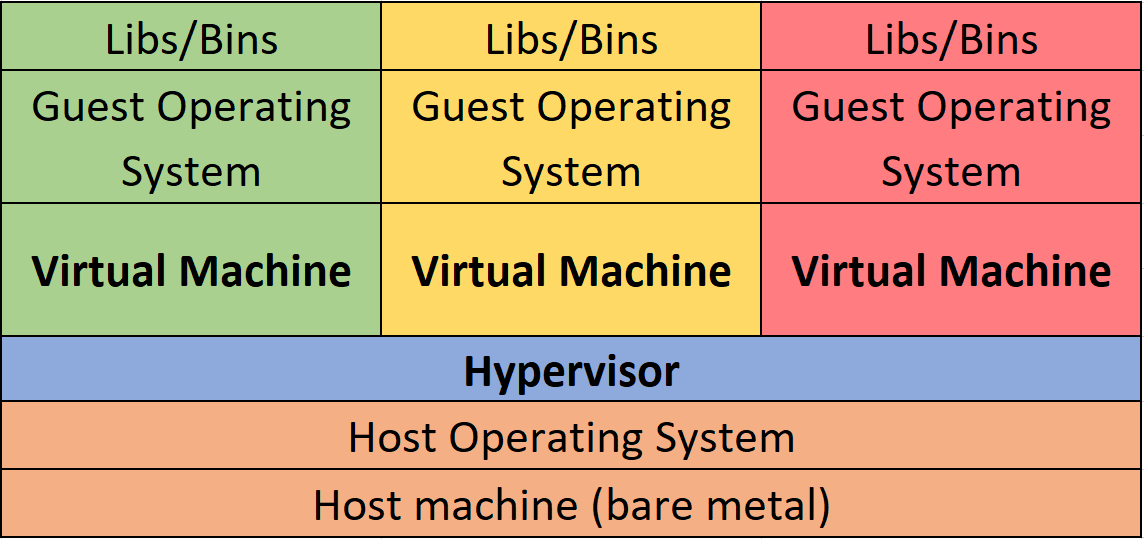
\includegraphics[width=0.95\textwidth]{./analysis/VMdiagram.PNG}}
\centering
\end{figure}

\section{Choosing a Virtualisation Platform}
There are a number of different hypervisors available for the practical work we will be doing in this project. Each one has different benefits and compromises. With this in mind, we must go through a process of deciding which technology we want to use to support our infrastructure. It is important to pick a virtualisation platform that is used in the industry I am aiming my research towards (that being SMEs with a need to host servers internally).

\subsection{VirtualBox}
VirtualBox is a popular virtualisation platform provided by Oracle \citep{VirtualBoxOracle}. It includes virtual network cards that allow virtual machines to communicate with each other \citep[1.3. Features Overview]{VirtualBoxManual}, which is beneficial to us when hosting inter-connected servers. It also offers various networking options that allow for internal networks, as well as forwarding data onto a real interface \citep[6.2. Introduction to Networking Modes]{VirtualBoxManual}. This means servers could be connected in a virtual network, or could forward their traffic to a hardware network interface card, which means we can do our testing, and also apply the findings to real-world networks.

However, VirtualBox has recently come under scrutiny for a reduction in stability of their virtual machines, with some users reporting crashes, and slow-downs in operation \citep{bradford_2020}. When wanting to find a good contender for a comparative piece of research, it is important to stay away from something that could result in unfair results. As using VirtualBox may lead to slow-downs that are not a result of the Virtualisation technology itself, it wouldn't be a fair comparison to compare VirtualBox Virtualisation with a Containerisation, as differences in results could actually stem from something other than purely the raw performance we would expect to see on a virtual machine. VirtualBox is also considered a desktop-virtualisation package primarily, and doesn't offer any server-specific virtualisation packages, which also seems unfair given the great number of other virtualisation options available that \emph{do} have server-oriented versions.

\subsection{Hyper-V}
Hyper-V is a hypervisor product developed by Microsoft. Unlike VirtualBox with its lack of server-oriented packages, Hyper-V has two primary versions (Though there are sub-versions within these), one is a server-specific version designed to work on windows server, and the other is a stand-alone version designed to work on windows desktop environments (Like windows 10) \citep{HyperVIntro}.

Hyper-V also supports three different virtual switch methods, those being ``Private'' (traffic can flow between VMs only), ``Internal'' (traffic can flow between VMs and the host, alternatively NAT can also be configured to allow access to the internet), and ``External'' (traffic is bound to a physical NIC and forwarded onto a real-world network) \citep{HyperVSwitches}. For our testing, we would be able to use the internal switch with NAT so that our VMs could access the internet. Results could then be applied to real world networks using the external switch.

Like VirtualBox it supports multiple Operating Systems, including Linux (which we will need for our testing, see Section \ref{sec:LAMPsystem}). However, wider Operating System support isn't one of Hyper-Vs strong points \citep{HyperVVMwareComparison}, and this support for `Linux' is actually only actually full support for specific Linux operating systems, such as Ubuntu, Debian or CentOS \citep{LinuxHyperVSupport}. Whilst this wouldn't necessarily be a problem for \emph{our} tests, it does somewhat damage our ability to use it as a recommended system, as some end users and organisations might not be able to make use of it due to requiring specialist operating systems that are simply not supported within Hyper-V.

\subsection{VMware}
VMware is a well-known virtualisation package and hypervisor. Whilst Hyper-V had a relatively small guest OS support; VMware has a relatively huge support base for various different Operating Systems \citep{HyperVVMwareComparison} \citep{VMwareCompatabilityGuide}. This is important because it ensures that if relevant organisations want to use this research, they have a greater chance of being able to move over \emph{other} server functions that aren't necessarily covered in this report.

VMware provides hypervisor technology for a number of different applications, including server infrastructure virtualisation and desktop virtualisation. The core hypervisor technology across these different versions however, remains much the same \citep{VMwareProductGuide}.

The other key issue picked up with other virtualisation packages (namely VirtualBox) was stability. VMware on the other hand, is considered very stable \citep{pavlik2012supervisory}, and is certainly more stable than VirtualBox \citep{bradford_2020}. This ensures that our results are reflective of virtual machine performance, and not shifted by hitches in the hypervisor programme.

\subsection{Decision}
With the above in mind, in order to provide virtual machines for testing in this research we will be using VMware Workstation Pro \citep{VMwareWorkstationPro}. This choice comes for a number of reasons, one being because it is one of the leading virtual machine hypervisors for the desktop environment \citep{BestVirtualisationSoftware}, which makes application to real-world server infrastructure much easier. Another main reason we decided to use VMware is because of its many versions despite using the same technology across said versions. As a result, data we get from this research in relation to VMware Workstation Pro, should be applicable to other VMware applications, such as VMware ESXi which is used in enterprise server applications \citep{esxivmware}. This crossover between server variants and the desktop variant of VMware gives us a unique advantage as we can easily create and manage virtual machines in our desktop testing environment, whilst not damaging the credibility of our results.

VMware also provides us the exact network options we require, whilst also giving us the ability to alter and change networks using the built-in network manager \citep{VMwareNetChange} (this is important for section \ref{TheNetworkSynthesis} later in this report).

\chapter{Review of Containerisation}
\label{chap:containerisationReview}

\section{Terminology \& Definitions}

\subsection{Containerisation}
\label{sec:containerisation}
Containerisation has become the de-facto term to describe what has also been described as OS-level virtualisation \citep{hogg_2014}. For the purposes of this report, I will be referring to this technology only as Containerisation, and each individual instance shall be referred to as a container (instead of virtual machine). This is the same approach towards defining containers as taken by Dua et al \citep{dua14} who have made their own distinction between Containers and Virtual Machines in much the same way that we have.

The next sections will cover what containerisation is, and how it works. This is important so that the difference between virtualisation and containerisation is fully realised.

\subsection{Container Engine}
\label{Container Engine}
What a hypervisor is to a virtual machine, a container engine is to a container. A container engine sits on the base operating system, much the same as a hypervisor. Where a difference is found however, is in the way it interacts with said base operating system.

Whilst a hypervisor works by running a full operating system on top of the existing one, and then managing the transfer and allocation of resources from there, a container engine works without that upper operating system by using the host machine's operating system as the OS component for each container. Segregation of containers and resource allocation is still managed by the container engine, so that each container is allocated separate and isolated resources. This can be done dynamically or be static, depending on the use-case (much the same as virtualisation).

This effectively removes part of the overhead that was previously required for each virtual machine. In theory, this should allow for improved performance over Virtual Machines, especially when system resources are scarce or under a large load.

Figure \ref{fig:ContainerDiagram} shows diagram that illustrates how the containers and container engine work in relation to the host machine. When compared with the diagram in figure \ref{fig:VirtualisationDiagram}, we can see that containers have far less overheads in comparison to virtual machines.

\begin{figure}[H]
\caption{Diagram basis taken from Jenny Fong (Docker Blog)\citep{ContainerDiagram}}.
\label{fig:ContainerDiagram}
\fbox{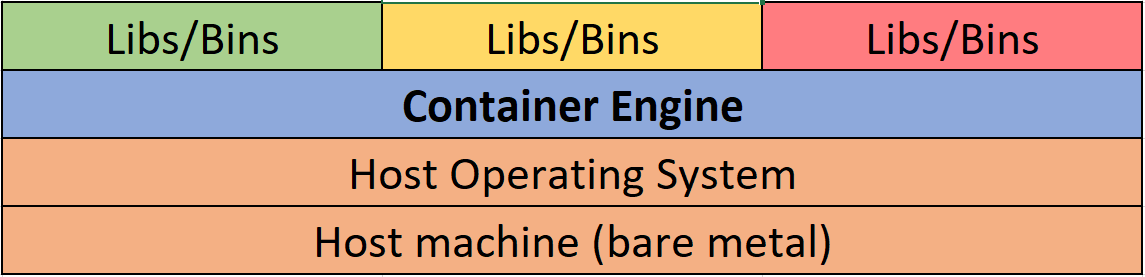
\includegraphics[width=\textwidth]{./analysis/CONdiagram.PNG}}
\centering
\end{figure}

\section{Choosing a Containerisation Platform}
Whilst containerisation is still relatively new, there are still a few options for us when deciding which containerisation package to use. Similarly to how we decided which virtualisation package we are using, we need to do a little bit of analysis into the various alternatives available to us, and decide which one is best for our own uses.


\subsection{FreeBSD Jails}
FreeBSD is an operating system that descended from the Unix family, much the same way that Linux did. BSD relates to ``Berkley Software Distribution'' which was a (now defunct) Operating System. When BSD stopped being supported in 1995, a number of organisations continued developing their own versions of BSD. By 2005, FreeBSD was the most popular by far \citep{BSDSurvey}, and remains one of the most popular versions today.

FreeBSD has been used to produce systems for a number of different use cases, but of those, server infrastructure is the one that would make most sense to our research. FreeBSD can support a number of different server functions, such as DNS, Web and FTP servers \citep[Section 1.2.1.]{FreeBSDHandbook}.

Whilst not named ``containers'' by the FreeBSD team, what FreeBSD calls Jails \emph{are} a form of OS-level virtualization (which for our research, we are considering to be containerisation, as discussed in subsection \ref{sec:containerisation}). Jails segregate functions logically, but still use the base kernel and Operating System in order to function. A unique benefit to FreeBSD jails is benefit that a long history of support provides. FreeBSD Jails were first introduced in 2000 \citep{FreeBSDJailRelease}, and have received continuos updates and development cycles, making it one of the most sturdy container systems to date.

However, to make use of FreeBSD Jails, it is a hard-requirement that the Operating System and Kernal \emph{must} be FreeBSD. There is no way of supporting FreeBSD Jails on anything other that FreeBSD as it is baked into the FreeBSD environment itself. This takes away from the autonomy of businesses that may want to use the product, as they can't choose to use a different operating system (such as windows or Linux). This could also be a problem as an organisation might see the outcome of this research and decide they want to move to a container-based system, only to be stopped in their tracks due to being unable to integrate the FreeBSD Operating System in their current system.

\subsection{LXC}
Another option is LXC, also known simply as `Linux Containers', it was released in 2008. LXC makes use of Linux 

\subsection{Docker}%NEED TO ADD MORE CONTAINER ALTERNATIVES HERE, MENTION JAILS WHICH ARE SIMILAR
An increasingly more popular implementation of container technology is a software known as Docker. This software is primarily used by (and aimed at) developers, who can use the platform to quickly create and deploy applications in container environments for testing. The use of containers is supposed to make managing these applications much easier, as it ensures compatibility along the whole development process. For example; a developer can code a program, then pass their code \emph{and} container onto QA who can test the code in exactly the same environment \citep{whydocker}.

Datanyze (a technology market usage group) report that Docker is currently the second most used Containerisation platform, with 25.34\% market share in Containerisation \citep{datanyze}. 
\section{Using Docker}
\subsection{How Docker works}
\label{subsec:docker}
Docker's Container engine is aptly named Docker Engine, and utilises a client-server architecture \citep[Section: Docker architecture]{DockerOverview}. The server portion of the Docker System is known as the `docker daemon', the Client uses a command line interface to interact with one or more docker daemons. The client and daemon communicate using a `REST API' \citep[Section: The Docker daemon]{DockerOverview}. REST (Representational State Transfer) provides an architecture for web services \citep{W3Architecture2004} that allows them to communicate over HTTP. The protocols within REST are stateless, this means there is no set `state' or session control within the protocol; each command sent to a daemon can be understood as it is, without the need for any outside context to the command being sent.

The Docker Daemon manages `Objects' \citep[Section: Docker objects]{DockerOverview} required for a full Docker system. 'Objects' refers to the containers, the images (Docker images are the instruction sets for Docker containers, not to be confused with OS images, though often the Docker images will include which OS image is to be used).

Docker images are stored in a Docker Registry \citep[Section: Docker registries]{DockerOverview}. By default, the registry is configured to use "Docker Hub" which is a public, open registry that already contains a large number of complete images for use. This registry can be changed however, to point to any location. This behaviour allows a registry to be setup part of a network, and the images can then be 'pulled' or 'run' from the registry using the "docker pull" and "docker run" commands\citep[Section: Docker registries]{DockerOverview}. An image can also be configured on a live container, and then that image pushed to the registry using the "docker push" command \citep[Section: Docker registries]{DockerOverview}.


Docker is written using the 'Go Programming language' \citep[Section: The underlying technology]{DockerOverview}. Go is developed and maintained by Google on an open source liscense, and is roughly based on the C programming language\citep{GoAncestors}. Being based on C gives the programming language the same benefits of any other low level language, being able to make use of functions that are integral to the kernal and operating system. Where go differs is that it is also designed to be be more intuitive and "clutter free" \citep{GoPrinciples}.

\subsubsection{Namespaces}
Docker makes use of a feature of Go that allows further use of a linux kernal feature known as namespaces \citep[Section: Namespaces]{DockerOverview}.
When new containers are created, a set of namespaces are created sepcifically for that container. This means that programs that might otherwise be considered by the kernal to be entirely sperate, are processed together, and vice versa. This in turn allows multiple containers to run processes in isolation that otherwise would have been processed by the kernal together, and also process a number of actions as one whole unit, that otherwise would have been considered seperate tasks to the operating system. This is key to the function of containers, as it allows each container to process tasks as sperate entities, but make use of the same kernal and operating system across all containers.

\subsubsection{Control Groups}
Control groups is another feature of the linux kernal used by Docker. Control groups allow hardware resources to be segrated in a way that limits and further isolates them \citep{corbetControlGroups}. In docker, this is used to segregate parts of memory, logical processors, drive space and network access so that there is no crossover in hardware utilisation between different containers. This is similar to how a hypervisor would segregate resources, but instead this is managed entirely by the kernal.

\chapter{Comparisons Between Virtual Machines and Containers}
\section{Research comparing both methods}
\label{ComparisonStudies}
\subsection{To support PaaS}
Research has already been conducted comparing containers and virtual machines, such as Dua, et al.'s study into using containerisation and virtualisation in PaaS (Platform as a service)\citep{dua14}. In this study, it was concluded that containers performed better in almost every way for online applications, but they also concluded that adoption of containers was still relatively low, and that there were some issues with standardisation in the field\citep{dua14}. That study was conducted in 2014 however, so a lot could have shifted by now. 

Since that study took place, we have had a whole host of changes that could have had substantial impact in the field. For example; since this study, Microsoft has released Windows 10 (2015)\citep{WindowsIntro}, and then later, Windows Subsystem for Linux (WSL), which provides the ability to run Linux applications on Windows\citep{wslrelease}. WSL2 has also been released, using a real Linux kernel\citep{wslkernel}, and has been adopted by container applications such as Docker\citep{Dockerwsl}, allowing them to run better on windows machines, could this be the start of the standardisation that Dua, et al. were looking for?

\subsection{A more recent review}
In 2019, Watada, et al. did a review of containerisation and found that containers were faster in virtually every deployment when compared to tradition virtual machines\citep{watanda19}. This study was thorough in looking at the workings of various Virtual Machine and Container technologies, but most of these were tested on cloud applications, such as AWS (Amazon Web Services). The results in this study focused more on seeing how containers were already deployed in working environments\citep[VII.]{watanda19}, and the benefits of using them in those situations. Whilst recommendation were made as to where containers should and shouldn't be used, the study makes mention that complex networking is difficult to achieve using containers\citep[VIII. A.]{watanda19}.

The main issues mentioned by Watanda, et al. regarding complex networking with containers is IP address application, mentioning that most most containers make use of NAT networking\citep[VIII. A.]{watanda19}. It is mentioned, however, that NAT networking can be avoided by assigning individual containers directly to host network interfaces\citep[VIII. A.]{watanda19}.

\section{Full Virtualised/Containerised Networking}
\subsection{Virtual networks}
We have already discussed the many applications of virtual machines, and among these is the ability to run multiple networked VMs on the same hardware, keeping various parts of the network logically separate. One example of this is VMware's network manager, whereby virtual machines can be made to appear as separate entities on a physical network\citep{VMwareNetChange}, whilst all sitting on the same base machine.

\subsection{Containerised Networks}
The studies and research mentioned above in section \label{ComparisonStudies} show that containers, in most situations, are faster than Virtual Machines. Where containers are said to fall down is their ability to interface and be deployed easily in real world situations. This is why most SME's still rely on Virtualisation for a large portion of their network infrastructure, despite the fact they could probably prolong their hardware, or get more raw power from existing hardware by moving to containers.

In this report we will be aiming to create a typical network topology that could easily be deployed on virtual machine infrastructure, and then, we will be applying this same exact topology to a containerised network, and then measure that actual performance benefits in order to generate a recommendation to those that are still using virtual machines to host their infrastructure.

\chapter{System design and definition}
\label{SystemDesignDefinition}

\section{Maintaining scientific method}
To ensure that results are scientific, variables must be controlled between both of the systems. The first step in this, is ensuring that the topology and configurations for both systems are the same. This can be done by copying the configuration files from one system to the other, ensuring that the system works in the same way for both systems. As the underlying operating system should be a version of Linux for both the virtual machine and the Docker system, this should be relatively easy.

To further ensure that variables are controlled, we need to ensure that the same benchmarks are maintained throughout the testing process, when being used on the \emph{same part of the system}. This means that if one benchmark is used to measure, for example, network latency on a web-server, then the same benchmark should be used to measure the network latency on that same web-server on the mirrored system. It may be necessary to use different benchmarks across the whole system, but this is acceptable as long as all testing is done to a parallel across both systems. The benchmarks to be used will be discussed in more detail in section \ref{sec:Benchmarking} (Benchmarking).


\section{LAMP System}
\label{sec:LAMPsystem}
I will need to make sure that the test system is as accurate to a real-world system as possible. To do this I will be employing a LAMP topology for both the Docker system and the Virtual Machine system. LAMP is the acronym for Linux, Apache, MySQL and PHP. Whilst this can technically be run all on one system, it is common to separate various functions out onto different machines (logically or physically), this generally makes management of these systems easier.

For the Linux section of the LAMP topology, I will be employing Ubuntu Server as it is headless which resulting in a lower overhead, and because Ubuntu is one of the most widely used Linux operating systems for website infrastructure as of 2021 \citep{w3techUbuntu}. Ubuntu even has its own images stored officially on Docker hub, which is updated regularly to stay in line with Ubuntu's Long Term Service version \citep{ubuntuDocker}. Some of the images hosted on Docker Hub by Ubuntu \citep{ubuntuDockerProfile} are already configured to contain some of the parts required for the deployment, such as Apache2 and MySQL. These may be useful when implementing a Docker setup in the synthesis of this report, though for the sake of ensuring a fair-test, I may instead push images to docker that use the exact setup used by my virtual-machine testing. This could remove a possible source of extraneous variables from the testing.

\section{Benchmarking}
\label{sec:Benchmarking}
Benchmarking software and tools are designed to create a standard output measurement for performance of a computer-based system\citep{fleming1986}.

There are a  number of benchmarking tools available, but for this research these can be split in discussion along lines of what they are designed to measure. That being said, the main split for this research is the measuring of computing performance, and of network performance.

\subsection{Computing Performance}
\label{computingperformance}
Computing performance in this case relates to the performance as a result of the computers ability to process information, and at what rate. Whilst this is tied directly to the processor, RAM, and other hardware, the overhead of the Operating system can affect these components and as a result, have a large affect on the performance of a system. This effect is known as `operating system overhead'. Based on previous research on containers and virtual machines it can be hypothesised that in this research, the total Operating System overhead for a container-based system will be smaller than that of Virtual Machines \emph{(when using the same operating system)}. This is due to the way that containers utilise one OS for their function (as discussed in subsection \ref{Container Engine}).

\subsection{Network Performance}
Further to the Computing Performance; Networking Performance is the measured performance on the network between various nodes. These nodes are the servers, clients and other infrastructure that are configured to receive and send traffic on a network. One of the best ways to measure network performance is delay. Compute performance may change the network delay in some areas, but not all. To explore this, we should further break network delay into its four main components:
\begin{itemize}
  \item Processing Delay: The amount of time it takes for a node (router, server, client, etc) to process the header of a packet \citep{ProcessingDelay}. This is usually affected by the CPU performance, which is linked to the compute performance as discussed previously.
  \item Queuing Delay: The time spent after being processed or produced by the node, and then actually being pushed onto the line \citep{QueuingDelay}. This is called queuing delay, as this delay is most usually due to other data already being pushed out onto the line. As a result, our data is waiting in a 'queue' behind other data, waiting to be pushed onto the line. This is affected by the amount of traffic being sent from a node, along with the speed at which the node can process multiple packets. This does tie in with Computing performance.
  \item Transmission Delay: The amount of time it takes for a node to 'push' packets (bit by bit) onto the line \citep[Chapter 7]{chen2005}. This delay is a result of the bandwidth on a line, and as a result, the change in transmission delay between virtualisation and containerisation can't be hypothesised. This is due to differences in the way that both methods manage network traffic. There is no physical line between the servers, so differences in bandwidth are entirely down to the relevant solution (Containerisation, or virtualisation).
  \item Propagation Delay: The time it takes for packets to travel over a line/medium (such as copper cable) \citep{PropogationDelay}. This could be affected by the the change from virtualisation to containerisation, however, this would be down to the individual ways that each of the solutions I choose manage network traffic between logical machines. As such, I can't generate a hypothesis for how this would be affected, much the same as Transmission Delay.

\subsection{Other key findings}
Whilst the purpose of this project will be primarily to find differences in speed between the two methods, there may be other performance, or even logistical improvements of one over the other. The final output from this research should be a recommendation to those that might be considering using containers in order to run their infrastructure, so whilst performance might be the key focus of this report, I will ensure to mention in evaluation anything else that could be considered important to those that might be looking to containerisation as a 'step forward' for infrastructure. For example, in subsection \ref{subsec:docker} (Docker) I discuss the Docker Hub, which is an public repository of images that anyone can push to or pull from. This system might make the deployment of containers easier than the deployment of virtual machines, so whilst this isn't directly related to the performance of the system itself, it may be worth mentioning as a possible point of interest.
\end{itemize}

We can see from exploring these various types of delay on the network, that network delay can be directly tied to Computing Performance in \emph{some} areas. As a result of this, it could be expected that the changes to overhead, and the possibility of streamlining processes as discussed in chapters \ref{chap:virtualisationReview} and \ref{chap:containerisationReview}.

\section{Requirements List: Infrastructure}
\label{Requirements:infrastructure}
To create a realistic web infrastructure, a number of services will need to be implemented across 

\subsection{Webserver}
\label{subsec:webserver}
The network will contain an intranet website in order to best simulate the intranets that are often operated by enterprises of various sizes across many different areas. Intranets are an integral part of a large number of businesses, as aim to serve as a central node for a large number of operations within businesses. These intranets can often host a number of important services for day-to-day working of a business \citep{jacoby2005critical}, such as time-sheet and clock-in access, information sharing, and policy documentation hosting, to name a few.

\subsubsection{Apache}
\label{apacheserver}
The Apache HTTP server (Apache) is an open source HTTP server software developed by the apache foundation. It is (as of current) the most widely used HTTP server in the world with 34.5\% of known websites using Apache to host their infrastructure\citep{ApacheUsage}. This makes it the perfect tool for simulating a real-world enterprise network, and should give fairly realistic results from benchmarks.


\subsection{DNS}
The architecture will require a DNS system in order to resolve hostnames outside of our own control (Recursive DNS), and to to maintain the control over the domains for the intranet discussed in \ref{subsec:webserver}. Secondary DNS servers will be configured to interact with clients, whilst the primary and authoritative server will be hidden from clients. Having secondary servers acts both as a way to load balance DNS requests from the clients, and to act as a redundancy should one of the servers fail.

It is important to mention that for the purposes of testing, Reverse DNS (rDNS) will also be configured \citep{rfc1035}. This service essentially converts from IP addresses to hostnames, and is useful for using test commands such as Ping and Traceroute. These commands wont appear in the testing, but will be useful for troubleshooting when the systems are being created.

The primary and secondary forwarding addresses for queries unknown to the primary DNS server will be Google's Public DNS servers. (8.8.8.8 and 8.8.4.4).

\subsubsection{BIND}
As the machines running the network infrastructure will be using Linux, the best fit for DNS architecture will be the use of BIND. This is because BIND is the de-facto standard for DNS on linux, and because it allows us to run the DNS server both as a recursive (for finding DNS queries for the outside network) and an authoritative (for managing the intranet domain) DNS server. BIND is maintained by the ISC \citep{ISCtimeline}, who also maintain a Docker Image for the application in docker hub.

\subsection{DHCP}
\label{DHCP Spec}
The network will also require a DHCP server in order to allocate IP addresses to clients.

\subsubsection{ISC-DHCP}
Another ISC solution\citep{ISCtimeline}, this will be used in order to manage DHCP. This service is simply known as ISC-DHCP and is another de-facto service in enterprise environments. These programs are in line with the testing I am doing, as they are commonly used in real world environments, which is where my research aims to replicate and implicate.

\subsection{MySQL}
\label{MySQL Server}
As discussed in \ref{sec:LAMPsystem}, a MySQL server will be used in order to host a database. There are a number of reasons an organisation might want to host a database on their internal network, such as storing employee information for access on the intranet. Databases can take a lot of resources to maintain, and are often an important part of key infrastructure. Any increase in database performance from virtualisation to containerisation would be a clear success, and a good reason to move over to containers over virtual machines. MySQL has its own Ubuntu Server Package, making the server portion of the installation easy.

\subsection{Clients}
Whilst not technically a service, the network will have to include at least one client in order to test that the services listed above actually work as intended. These sorts of internal networks are made entirely to serve clients, so without testing performance on the client end, the testing would be somewhat redundant. Ubuntu Desktop will be used, as it is also open source and can be deployed easily on both systems. The client machine used in testing will be a VMware machine so that it can interact with the network setup for testing. The same system resources will be allocated to this client for both testing environments, so whilst there will be an impact on the performance of the machine doing the testing, it should have the same impact on the host machine's system resources across both systems, and shouldn't change the legitimacy of the output.

\subsection{Topology Diagram}
\label{subsec:TopologyDiagram}
Figure \ref{fig:Topology} is a mock-up of what the final topology should look like logically. This will be subject to change throughout the synthesis section of this report, as findings are made and areas are adapted.
\begin{figure}[H]
\caption{}
\label{fig:Topology}
\fbox{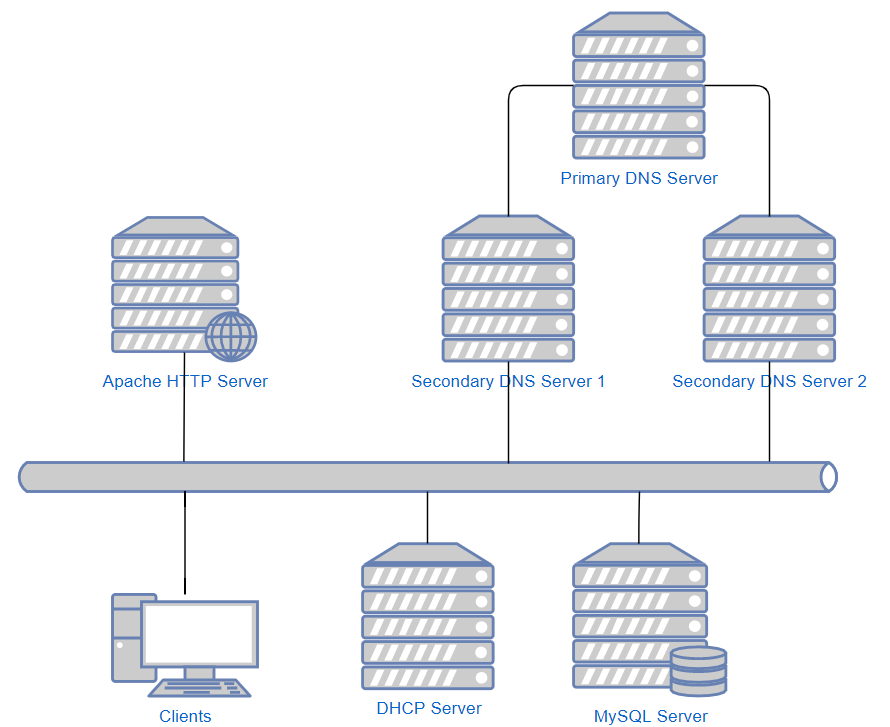
\includegraphics[width=\textwidth]{./analysis/Topology.PNG}}
\centering
\end{figure}

This topology should be replicated in the same way across both systems in order to ensure that the results are measuring exactly what is supposed to be measured.

The difference in setup here is that Docker containers are run from the command line on the host machine whereas VMware will be using the VMware workstation pro environment to virtualise a new operating system for each instance. 

\chapter{How will the system be measured}

\section{Requirements list: Benchmarks to be used}
\label{RequirementsListBench}
The system will need to be measured using standardised benchmarks in order to ensure that results are comparable.

To ensure that all elements of the system are measured, I will do four tests as follows.

\subsection{Test one - iPerf3}
iPerf is a tool used for measuring the total bandwidth achievable over IP networks \citep{iPerf3}. In this test, the throughput will be tested between the client and the Apache server, as realistically, this is the server that would receive the most traffic in a real deployment. It can be expected that any server to client bandwidth would be the same however, given that the connections are all virtual and should work much the same way, regardless of which server is being used.

Measuring throughput for the web server is important because a higher throughput should mean a greater number of users being able to use the website without long wait times for example.

\subsection{Test two - Sysbench MySQL}
Sysbench is a benchmarking tool that comes with a number of different tests for measuring processing, memory usage, Input/Output speed, and database performance\citep{sysbench}. Whilst the tool is extremely versatile, with tests for a number of different functions, the test that is of interest to this work is the 'oltp\_read\_write' test supplied. This test performs a number of random read and write queries and transactions to a pre-prepared MySQL database using OLTP (Online Transaction Processing), which is a system which facilitates small-scale, multi-user transactions and processes to a database\citep{oltpbenchmarking}.

This test will be performed on the MySQL server outlined in subsection \ref{MySQL Server}, with the client machine being used to send the queries and initiate reads and writes.

The output from this test should give the number of queries that were successfully performed, along with the total latency for each transaction that takes place. These measurements are important because lower latency and a higher number of transactions in the same amount of time in a real deployment would result in better load times for end users for any web pages that require database manipulation. Even databases that don't face any users could see benefit from increased performance however, as lower latency allows for greater workloads \citep{MySQLlatency}, which would allow heavier, more demanding work to be allocated.

\subsection{Test three - Namebench}
Namebench is an old and archived, but still fairly standard DNS benchmarking utility developed by Thomas Stromberg as part of Google's 20\% program \citep{Namebench}. The project is using the Apache Open-Source License, and is still available to download and compile for use on Linux.

The tool's original purpose was for testing DNS response times for multiple websites against well-known, public DNS servers. The output from the test was designed to give the user a good idea as to which servers to use as their primary and secondary DNS servers in order to achieve the best response times possible when browsing the web. However, the outputs given can also be extremely useful for testing internal DNS server speeds. For example; the average, maximum and minimum latency given for each server. When this test is done for both deployments (Docker and VMware) the outputs can be compared to determine which DNS architecture gives less latency.

DNS latency directly affects how quickly websites load, as time is needed to resolve the server address from the IP. Overstressed DNS architecture can result in larger query latency\citep{DNSlatency}.

\subsection{Test four - Apache JMeter and Performance measurements using Netdata}
Apache JMeter is an open-source application provided by the Apache Software Foundation designed to allow load-testing of various servers \citep{ApacheJMeter}. It was initially designed for testing of web-applications, and whilst it can now be used to test a number of different protocols, we will be using it for testing of HTTP/HTTPS.

JMeter is fully user customisable, but under a fairly standard and basic use, it allows for the simulation of a number of clients to a remote server in order to simulate what a different loads would look like if the server were to be in a real deployment\citep{masterjmeter}.

This test will be performed against the Apache server laid out in subsection \ref{apacheserver}, and as with the other tests, the client machine will be used to initiate the test, so that the traffic uses the network environment.

However, JMeter only gives performance results that are perceived by the clients that it simulates, for example, query latency. It doesn't show the impact on performance of the machine itself during these stress tests. So to measure the computing performance (as laid out in subsection \ref{computingperformance}), Netdata will be implemented to run on the host machine in order to monitor the performance metrics.

Netdata is open source software that is designed to pull numerous performance metrics such as CPU and RAM usage in real-time from nodes and end-points, whilst maintaining as small of a footprint on that node as possible \citep{Netdata}. These statistics are displayed in a visual 'dashboard' which display a number of charts showing usage. A key feature of this dashboard is the ability to export and import snapshots \citep{netdatadashboard}. This feature will allow a snapshot to be created for each scenario, allowing for historical access to the exact performance metrics from each test. This allows for in-depth analysis even after the testing has finished.